\subsection{Описание модели}
Структурная схема представлена на рисунке \ref{fig1:image}.

\begin{figure}[h]
	\begin{center}
		{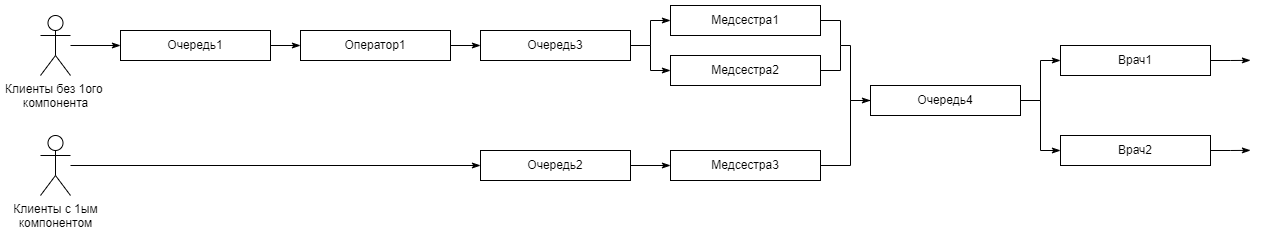
\includegraphics[scale = 0.37]{img/struct.png}}
		\caption{Общая схема}
		\label{fig1:image}
	\end{center}
\end{figure}

\begin{figure}[h]
	\begin{center}
		{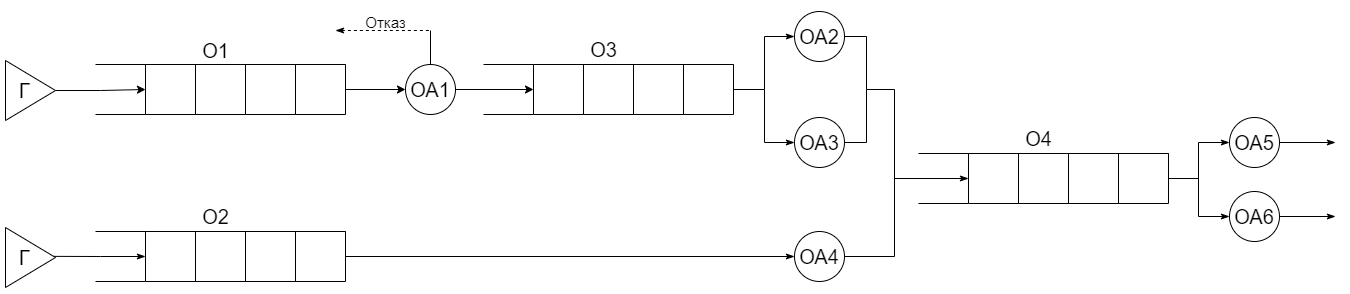
\includegraphics[scale = 0.37]{img/schema.png}}
		\caption{Структурная схема}
		\label{fig2:image}
	\end{center}
\end{figure}

\newpage


Время обработки клиентов подчиняется закону равномерного распределения. 
%
В состав модели входят: 
%
\begin{itemize}
	\item ОА1 -- оператор;
	
	\item ОА2, ОА3, ОА4 -- медсёстры, первые две отвечают за первый компонент, третья -- за второй.
	
	\item ОА5, ОА6 -- врачи.
\end{itemize}

\textbf{Переменные и уравнения имитационной модели}  

\textbf{Эндогенные переменные}: время обработки клиентов оператором, медсёстрами и врачами, время моделирования.

\textbf{Экзогенные переменные}: число обслуженных клиентов и число клиентов, получивших отказ, максимальные длины очередей.

